\documentclass{article}

%### Hacer uso de símbolos extra ###
\usepackage{latexsym,amsmath,amssymb,amsfonts}

%### Cambio de la fuente del documento###
\usepackage{mathpazo} %palatino

%### Incluir Graphicos ###
\usepackage{graphicx}

%### Comandos especiales para TABLAS ###
\usepackage{multirow, bigstrut}

%### Hiper referencias y ocultando el link (hidelinks) ###
%\usepackage[hidelinks]{hyperref}
\usepackage{hyperref}

%##########################################
%Formato archivo.tex, entradas de teclado
%solo dejar uno de los dos archivos activados
\usepackage[utf8]{inputenc}
%\usepackage[latin1]{inputenc}
%###########################################
\usepackage[T1]{fontenc}

%Título
\title{LuaBot\\Plataforma de Programación Orientada a la Robótica y Domótica}

%Author
%\author{Apellido, Nombre ~Código:~123\\
 %       Apellido, Nombre ~Código:~123.}
%### Agregar fecha manualmente ###
%\date{mmm, dia, año}

\begin{document}
\maketitle
%\include{dir/arch}

LuaBot (Nombre provisional) es una plataforma que puede ser usada en 
robótica, domótica u otros fines donde sea necesario automatizar un proceso
y pueda intervenir la electrónica.

Consta tanto de un hardware y un software, ambos de tipo 
\textit{open source}\footnote{Así se le conoce al hardware y software 
desarrollado y distribuido libremente. Para conocer más, puede visitar los
siguientes enlaces: \url{http://www.oshwa.org/definition/spanish/},\\ 
\url{https://opensource.org/osd} y \\
\url{http://www.gnu.org/philosophy/free-software-for-freedom.es.html}}. 

LuaBot es pensado como una herramienta que facilita la programación de 
tareas que necesiten ser automatizadas y/o tele-operadas incorporando
elementos básicos para tal fin, además, evita al usuario final la 
engorrosa tarea de aprender un lenguaje de programación, haciendo que éste
se ocupe principalmente del algoritmo a desarrollar.

\section{Estado del Arte}

\subsection{Hardware}

\subsubsection{Microcontroladores}

Los microcontroladores son computadoras en sí, eso se debe a que están
constituidas por partes que tiene un computador de propósito general
(portátil o computador de mesa) como lo es una unidad de procesamiento
central (CPU), memoria principal (RAM) memoria secundaria (ROM), y 
periféricos, sin embargo, se diferencias de ellos por su arquitectura. 

Y al mencionar la arquitectura se debe saber también que existen dos
grandes tipos de tecnologías \footnote{Una información más precisa la puede
		obtener del libro \href{https://books.google.com.co/books?id=N7u2x4LyJ7UC\&pg=PA8\&dq=harvard+von+neumann\&hl=es-419\&sa=X\&ved=0ahUKEwjCrOKkus_LAhVCQSYKHVBGB8gQ6AEIHTAA\#v=onepage\&q=harvard\%20von\%20neumann\&f=false}{Sistema de Procesamiento Digital}} 
: En primer lugar la Von Neumann la cual es muy
usada por computadoras personales; en esta, la filosofía es usar un solo bus
de direccionamiento de información solo que multiplexado, hacer uso de ésta
arquitectura minimiza los costos de desarrollo, ya que usa menos elementos
pero aumenta el tiempo de ejecución de procesos. En segundo lugar está
la tecnología Hardvard que a diferencia de la primera tiene buses 
independientes para la memoria principal como para la memoria secundaria
(memoria de programa). A pesar de que la tecnología Hardvard usa más
elementos que aumentan los costos de desarrollo puede hacer tareas con
mayor velocidad a comparación de la Von Neuman. Esto hace que existan
computadoras de propósito general (hacen muchas tareas) y otras de
propósito especifico (como los microcontroladores), aunque con el tiempo la
tecnología a logrado que se optimice el espacio del dado del semiconductor,
haciendo que éste paradigma desaparezca.

Los microcontroladores en general, se desarrollan con la tecnología hardvard
ya que no requieren de tanta memoria o procesos complicados, pero si atender
tareas de tiempo real, cosa que un computador personal no puede hacer en
general.

Existen diferentes empresas populares que se encargan de producir 
familias de microcontroladores las cuales se diferencian por arquitecturas
en el tamaño del bus, capacidad de memoria (RAM, ROM), velocidad, 
prestaciones en sus periféricos \footnote{En el libro: 
		\href{https://books.google.com.co/books?id=ODenKGOHMRkC\&pg=PA149i\&dq=perifericoi\&hl=es-419\&sa=X\&redir_esc=y\#v=onepage\&q=peroperiferico\&f=false}
{Microcontroladores: fundamentos y aplicaciones con PIC} se hace referencia
al uso de periféricos, pero señala que éstos son externos, cosa que no es 
precisa, un periférico también puede estar introducido en el encapsulado 
del microcontrolador, como es el caso
de los convertidores A/D o los PWM.} entre otros. Pero hablar de las
características de las familias que construye cada empresa está fuera
del alcance de este documento, sin embargo, a lo largo de la evolución de
ésta tecnología las empresas han marcado su modo de operación.

Para facilitar la comprensión, se mencionará tres grandes empresas: 
Microchip, Atmel y Freescale (antes Motorola).

\paragraph{Microchip} 

Es muy popular en el mercado de los microcontroladores con sus
PIC\footnote{PICmicro usado como controlador interfaz periférico}, en las
comunidades educativas es uno de los más usados\footnote{ 
La plataforma \textit{Pinguino} \url{http://www.pinguino.cc/}
se desarrolló bajo PIC y lo que la hace atractiva para la mayoría es la 
capacidad de emulación del comportamiento del Arduino, pues usa la mayoría 
de instrucciones, así, 
si se sabe programar en Arduino, se puede programar para \textit{Pinguino}.}
, inclusive en Colombia hace unos 12 años cuando se hablaba de 
microcontroladores no se mencionaban así, sino se denominaban simplemente 
PIC's (La mayoría de estudiantes no tenían idea que PIC solo se trataba de 
una familia de microcontroladores). Ésto era debido a que Microchip (como 
lo hace Windows) domina tal mercado.

Las comunidades de desarrollo de 
software centraron sus esfuerzos en crear aplicaciones que compilaran 
programas escritos en C\footnote{ C es un lenguaje de programación de 
medio nivel (antes denominado de alto nivel)} como es el caso de CCS creado
para el año de 1992. Para quien quería hacer uso de tal recurso debía pagar
una licencia y quienes no pudiesen pagar tal licencia podían hacer uso
de un lenguaje de programación denominado ASSEMBLER\footnote{El lenguaje 
		Assemble o ensamblador es un lenguaje de bajo nivel, eso quiere
decir que está más cerca de la máquina que del ser humano.}. Con el
surgimiento de otras empresas que no privatizaban las herramientas de 
compilación usuarios esporádicamente migraron a otras plataformas,
Microchip jactado por su popularidad se ha resistido a brindar herramientas
libres potentes (aunque ya entrega unas con limitaciones), sin embargo, en
la actualidad otras empresas han demostrado tener microcontroladores 
superiores a los ofrecidos por microchip.

\paragraph{ATMEL}

Ha demostrado ser superior a Microchip con sus microcontroladores 
AVR\footnote{Así como los PIC's los AVR son de 8 bits
de tamaño de bus, sin embargo, solo por mostrar una diferencia olgada
 mientras que microchip solo tiene un registro de trabajo AVR tiene 32.} y ARM\footnote{Son excepcionalmente poderosos para tareas de tiempo real
		 con sus arquitecturas de 32 bits a comparación de las de 8 bits,
 para dar un ejemplo de su aplicación los procesadores de éstos 
 microcontroladores son usados en la mayoría de celulares.} con sus bajos
 costos, potentes periféricos embebidos y rendimiento superior. Tal es así
 que el éxito de Arduino no se basa en la plataforma como tal, sino en 
 haber adoptado los AVR como su cerebro, sin embargo, se debe recordar que
 son arquitecturas de 8 bit no de 32 bits\footnote{Si el tamaño del bus
		 es mayor, corresponderá a hacer más tareas en paralelo, aumentando
 su velocidad de ejecución} comos los ARM. Al éxito del hardware de Atmel
 hay que agregar que ofrece gratuitamente un software de programación
 que optimiza los recursos de los microcontroladores denominado 
 \textit{Atmel Studio}\footnote{\url{http://www.atmel.com/Microsite/atmel-studio/}}. 

\paragraph{FreeScale}

Para microcontroladores, freescale maneja arquitecturas de 8 y 32 bits, pero
la intención de mencionar a freescale es debido a su patente, freescale
anunció hace un par de años la creación de microcontroladores a velocidades
de operación de 120 MHz\footnote{Son muy superiores si los comparamos con
las velocidades de operaciones comunes de microchip de 8 a 20 MHz.}, de 
tamaños diminutos de aproximadamente $1.9 x 2$ milímetros y otras 
características que se escapan de comparación por desconocimiento, aún así
FreeScale promete mucho.

\subsubsection{Sistemas Embebidos}

Para hablar de sistemas embebidos es difícil globalizar pues un sistema
embebido puede ser desde una calculadora, un celular o hasta el mismo 
microcontrolador, aún así, para contextualizar se mencionarán algunos
ejemplos populares de sistemas embebidos enfocados a la robótica y domótica.

\paragraph{RaspBerry pi}

Desde la aparición de Raspberry como una plataforma orientada a la educación
secundaria en el Reino Unido, el mercado se ha reorganizado en función
de poner a disposición sistemas pequeños capaces de ofrecer software de 
oficina o a fines con distribuciones linux 
cross-compiladas\footnote{Hace referencia a compilar programas desde una 
		maquina con una arquitectura distinta } que
poco o nada tienen que envidiarle a un PC que cueste al rededor de
\$1'500.000 de pesos con Windows 7, donde el valor del Raspberry es de unos
\$110.000 pesos.  Además hay que aclarar que Raspberry cuenta con 40 pines
de propósito general que pueden ser usado para robótica y domótica. En la 
imagen de la figura \ref{fig:raspberry} se hace referencia a el Raspberry pi 3 b+ que se puede
consultar en el sitio oficial \href{https://www.raspberrypi.org/}{Raspberry}
.


%Imagen para IEEE
\begin{figure}[hptp]
    \centering
    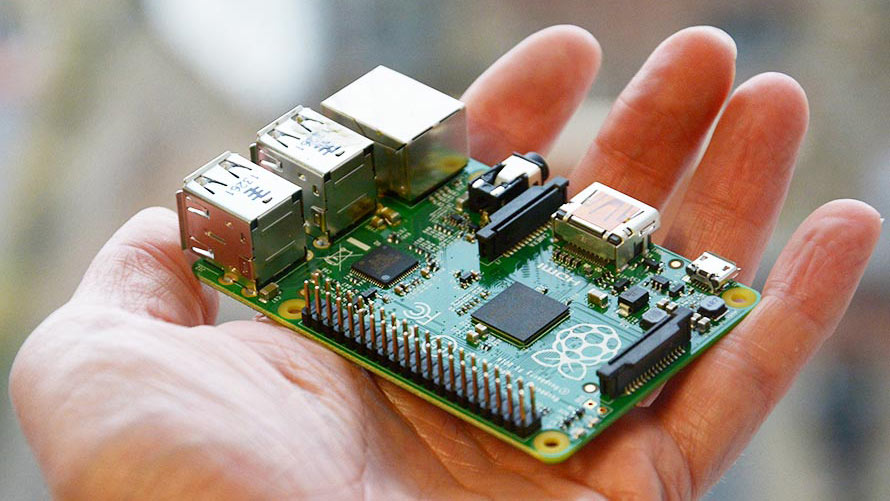
\includegraphics[scale=0.38]{imag/raspberryPi2.jpg}
    \caption{Computador a 1.2GHz 64-bit quad-core (cuádruple núcleo)ARMv8 
			CPU, 1G de RAM,wifi, bluethooth \dots en la palma de la mano.}
    \label{fig:raspberry}
\end{figure}
\smallskip

\paragraph{C.H.I.P}

C.H.I.P es una computadora en una tarjeta embebida que solo cuesta \$9 
Dólares, lo que lo hace extraordinariamente económico.\footnote{Se puede 
leer su documentación oficial en \href{http://docs.getchip.com/\#introduction
}{C.H.I.P.}} En ella se puede contar con servicios de Wifi, Bluethooth, 
salida de audio y vídeo para televisores, memoria interna de 4G, 
procesador de 1GHz, sistema operativo Linux y prestaciones para robótica
y domótica. Se puede adquirir también como un pocketchip el cual tendrá
un valor total de \$49 dólares, de esta manera obtendrá un sistema
Linux de bolsillo y para dejar en contexto la utilidad que podría llegar
a tener, podría sustituir calculadoras especializadas en graficación
y cálculos complejos las cuales cuestan al rededor de \$500.000 pesos.
En la figura \ref{fig:chip} se observa el pocketchip.


%Imagen para IEEE
\begin{figure}[hptp]
    \centering
    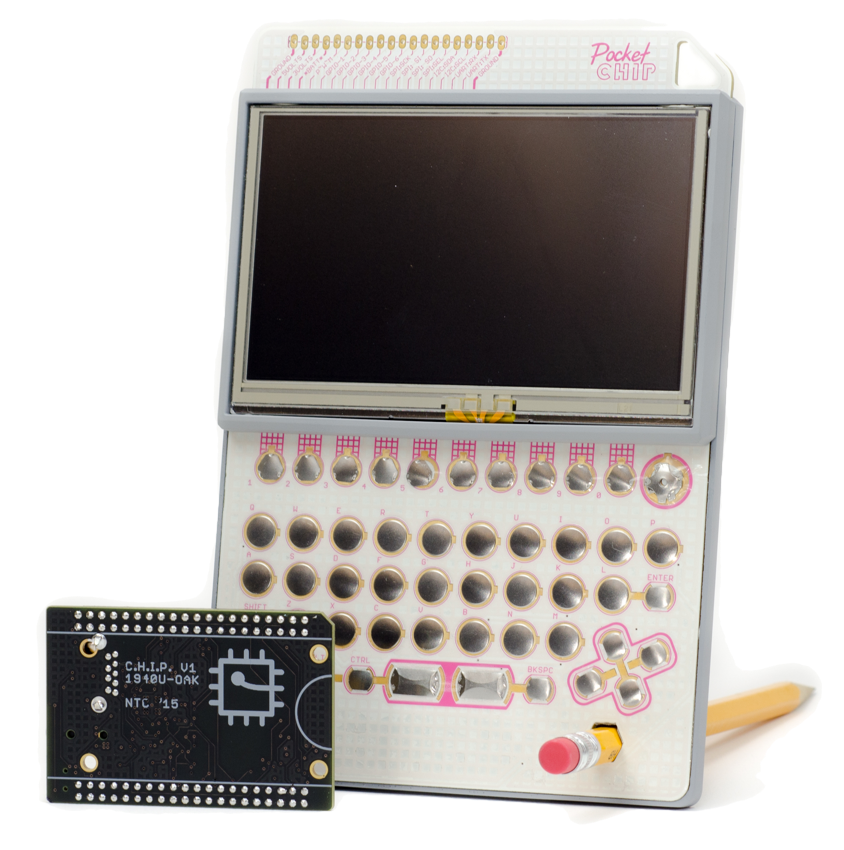
\includegraphics[scale=0.25]{imag/chip.png}
    \caption{Computador C.H.I.P con el pocketchip}
    \label{fig:chip}
\end{figure}
\smallskip

\paragraph{Arduino}

Arduino es una plataforma de desarrollo que consta de un IDE y una placa
con un microcontrolador generalmente  AVR, es muy conocido en el mundo,
soportando muchos periféricos a partir de librerías.

Arduino es usado para robótica como domótica a nivel educativo y 
profesional, llegando a ser uno de los más documentados en la internet con 
infinidad de ejemplos de aplicación
\footnote{Con el ánimo de crear controversia leer el siguiente 
 \href{http://dignal.com/porque-arduino-no-es-la-herramienta-correcta/}{link}
}. En la figura \ref{fig:arduino} se muestra un Arduino Due el cual tiene
un microcontrolador ARM. El costo de este Arduino es de 36 Euros (\$124.000
pesos) sin costo de envío.

%Imagen para IEEE
\begin{figure}[hptp]
    \centering
    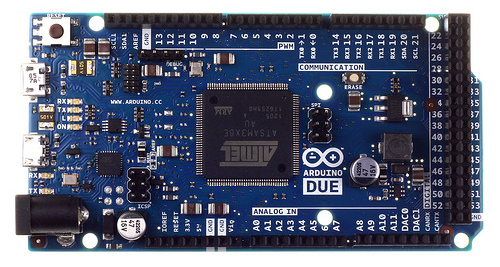
\includegraphics[scale=0.7]{imag/arduino.jpg}
    \caption{Arduino Due el cuál tiene un microcontrolador ARM}
    \label{fig:arduino}
\end{figure}
\smallskip


\subsection{Software}

\subsubsection{Lenguajes De Programación}

Los lenguajes han evolucionado a partir de diferentes paradigmas\footnote{
Un esbozo de lo que son los paradigmas de programación lo puede encontrar
en el libro: \href{https://books.google.com.co/books?id=rXU-WS4UatYC\&lpg=PR4\&dq=paradigmas\%20de\%20programacion\&pg=PA3\#v=onepage\&q\&f=false}
{Introducción a la ingeniería del software}}, 
como lo son estructurados, orientados a objetos, orientados a eventos 
entre otros. También los podríamos clasificar en dos grandes grupos:
los interpretados y los compilados\footnote{Una descripción de lo que
		es un compilador y un interprete lo puede ver en el libro:\href{https://books.google.com.co/books?id=nLMJsInMyBwC\&pg=PA8\&dq=compilador+e+interprete\&hl=es-419\&sa=X\&ved=0ahUKEwjy06Dj3NLLAhVFSiYKHblmCvkQ6AEIIDAB\#v=onepage\&q=compilador\%20e\%20interprete\&f=false}{Introducción a la programación. Teoría y práctica}}. 
Cuando un programa es compilado, es traducido una única vez al lenguaje 
máquina creándose el código objeto o código ejecutable, Mientras que cuando
es interpretado es traducido en tiempo de ejecución línea por línea.

Según \href{http://www.tiobe.com/tiobe_index?page=index}{Tiobe} los 10
lenguajes de programación más populares consultados en los buscadores
de internet (como google) a la fecha se presentan en la figura \ref{fig:lenguajes1}.

%Imagen para IEEE
\begin{figure}[hptp]
    \centering
    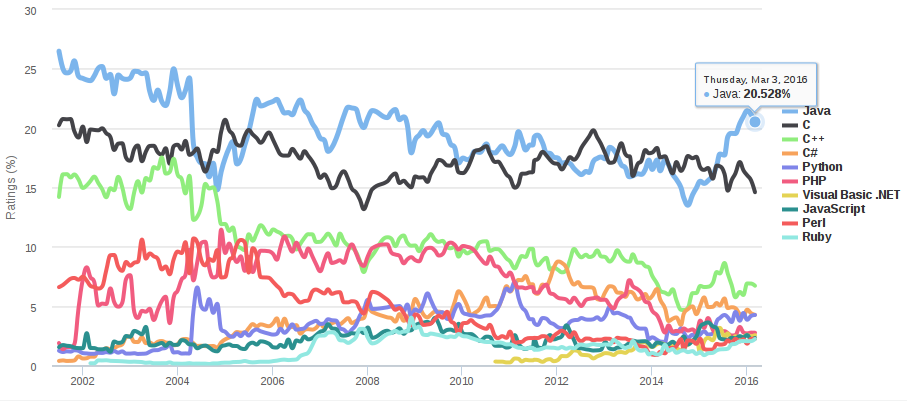
\includegraphics[scale=0.4]{imag/lenguajes1.png}
    \caption{Lenguajes de programación más populares, fuente www.tiobe.com}
    \label{fig:lenguajes1}
\end{figure}
\smallskip

Según \href{spectrum.ieee.org}{IEEE Spectrum} Los más populares para
sistemas embebidos se puede observar en la figura \ref{fig:lenguajes2}.

%Imagen para IEEE
\begin{figure}[hptp]
    \centering
    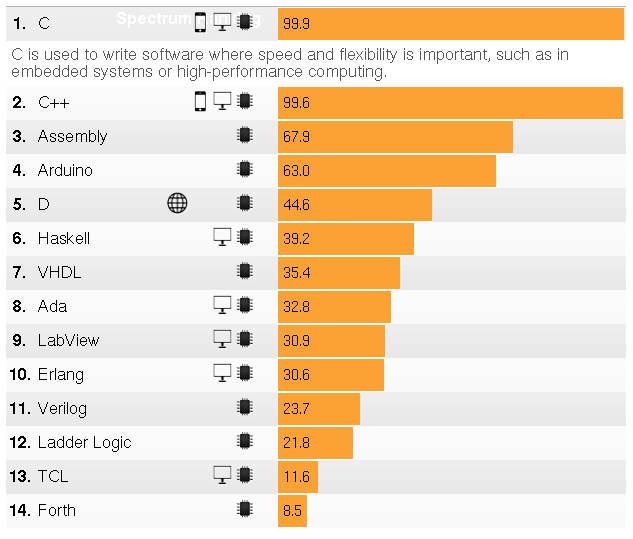
\includegraphics[scale=0.4]{imag/lenguajes2.png}
    \caption{Lenguajes de programación más usados para sistemas
	embebidos según IEEE Spectrum.}
    \label{fig:lenguajes2}
\end{figure}
\smallskip

Aún así, no se puede definir si un lenguaje es mejor que otro debido a que
pueden estar soportados en paradigmas diferentes y la optimización depende
también del uso.

\end{document}
